\chapter[Execução à nível de time]{Execução à nível de time}

Esse tópico representa as atividades e resultados obtidos pela equipe durante a execução do processo definido a nível de time.

\begin{figure}[H]
    \centering
    \label{identificarHistorias}
    \includegraphics[keepaspectratio=true,scale=0.6]{figuras/processoHistorias.eps}
    \caption[Identificar histórias]{Processo - Nível de Time - Identificar histórias}
\end{figure}


\section{Reuniões realizadas}
Foram realizadas três reuniões entre a equipe e o cliente para obter as informações necessárias do nível de time, todas presenciais.

\subsection{Reunião 01-Time}
\begin{itemize}
 \item \textbf{Data de execução:} 01/06/2016
 \item \textbf{Objetivo da reunião:} elicitar histórias de usuários do Business EP01.
 \item \textbf{Técnica de elicitação:} foi utilizada um conjunto de técnicas, sendo estas brainstorming e prototipagem.
 \item \textbf{Execução da técnica:} Nessa reunião a equipe utilizou a técnica de brainstorming com o auxilio da técnica de prototipagem. As features do EP01, foram utilizadas como temas para a realização da dinâmica.
 \item \textbf{Resultado da reunião:} Foi possível elicitar apenas as histórias das features: gerenciar informações acadêmicas, gerenciar um cadastro pessoal e controle de perfil de acesso. Sendo assim, o objetivo dessa reunião não foi alcançado. Os protótipos de papel feitos nesta reunião serão apresentados pelas imagens: \ref{prototipoPaper01}.
\end{itemize}

\subsubsection{Backlog das historias de usuário das features FT01 e FT02}
 O backlog a seguir foi elaborado a partir das reuniões com o \textit{Product Owner} até o presente momento da execução do processo.
 (Imagem que deve ser gerada com todas as USs das features 01 e 02)
 \ref{images}

\subsection{Reunião 02-Time}
\begin{itemize}
 \item \textbf{Data de execução:} 03/06/2016
 \item \textbf{Objetivo da reunião:} continuar a elicitação de histórias de usuário do Business EP01. Validar e priorizar as histórias de usuário elicitadas na reunião anterior \ref{reuniao01time}
 \item \textbf{Técnica de elicitação:} foi utilizada um conjunto de técnicas, sendo estas brainstorming e prototipagem.
 \item \textbf{Execução da técnica:} Nessa reunião a equipe utilizou a técnica de brainstorming para elicitar as histórias possíveis para as features Business FT03 e FT04. Com o auxílio da técnica de prototipagem para cla e produzir um entendimento melhor das histórias e seus critérios de aceitação.

 \item \textbf{Resultado da reunião:} a segunda etapa da execução da reunião foi concluída com sucesso, ou seja, as histórias que foram elicitadas foram validadas e estavam todas de acordo com os interesses do PO.\\
 As histórias para as features Business FT03 e FT04 também foram identificadas, entretanto, durante a eliciatação das histórias de usuário, a equipe identificou as features não estavam em total acordo com os interesses do PO.\\
 Devido ao fato de ter identificado mudanças nesta reunião, considerou-se que o objetivo da reunião não foi alcançado completamente.\\
\end{itemize}

\subsection{Gerência de mudanças}

 Foi identificada necessidade de mudança ao final da reunião 02 a nível de time. Essa mudança implicou na adição de novas features ao backlog e criação de um novo épico.
 Anteriormente, a Business FT03 \ref{backlogFeaturesPrograma} tratava das informações profissionais dos membros da empresa, só que o PO na verdade precisava que estas contivessem todas as informações externas a Zenit. Dessa forma, aquilo que seria tratado como informações profissionais tal como: participações em congressos, estágios, experiências profissionais, ele gostaria que também incluísse informações sem ser profissionais, tais como participações em projetos.
 E em relação a Business FT04 \ref{backlogFeaturesPrograma}, o que seria as informações de projetos internos e externos que os membros já participaram, na verdade isso seriam todas as informações internas a que o membro desempenha na Zenit.
 Como o time de requisitos havia elicitado todas as histórias de projetos e as histórias de informações profissionais, foi decidido que o time avaliaria as mudanças e voltaria a se reunir com o cliente para validar as mudanças.
 O artefato gerado pela execução do subprocesso de gerência de requisitos está no apendice X \ref{relatórioMudancas}.

\subsection{Reunião 03-Time}
\begin{itemize}
 \item \textbf{Data de execução:} 08/06/2016
 \item \textbf{Objetivo da reunião:} verificar se o PO aceita as mudanças identificadas na \ref{reuniao02time}. Elicitar histórias das features definidas no Business EP04 após mudança. 
 \item \textbf{Técnica de elicitação:} foi utilizada a técnica de brainstorming para identificar todas as possíveis histórias.
 \item \textbf{Execução da técnica:} com o tema de cada feature, foram jogadas ideias para histórias de usuário que atendessem a aquelas features.
 \item \textbf{Resultado da reunião:} o PO concordou com todas as mudanças feitas no backlog de features e épicos.\\
Todas as histórias foram elicitadas das features “Gerenciamento das informações dos minicursos”, ”Gerenciamento das informações sobre da área interna dos membros” e ”Gerenciamento das informações internas pessoais à Zenit”, assim o objetivo da reunião foi atingido.\\
Nesta mesma reunião, o PO fez a verificação e validação das histórias. Apesar de não estar no planejamento para esta reunião, como o PO compreendeu as atividades que estavam sendo realizadas, ele sugeriu validar as histórias, assim foi feita a verificação e validação pelo PO na mesma reunião.
\end{itemize}

\subsection{Backlog de Time}
 \ref{imagensdobacklog}

\section{Planejamento da sprint}
\begin{figure}[H]
    \centering
    \label{identificarPlanejar}
    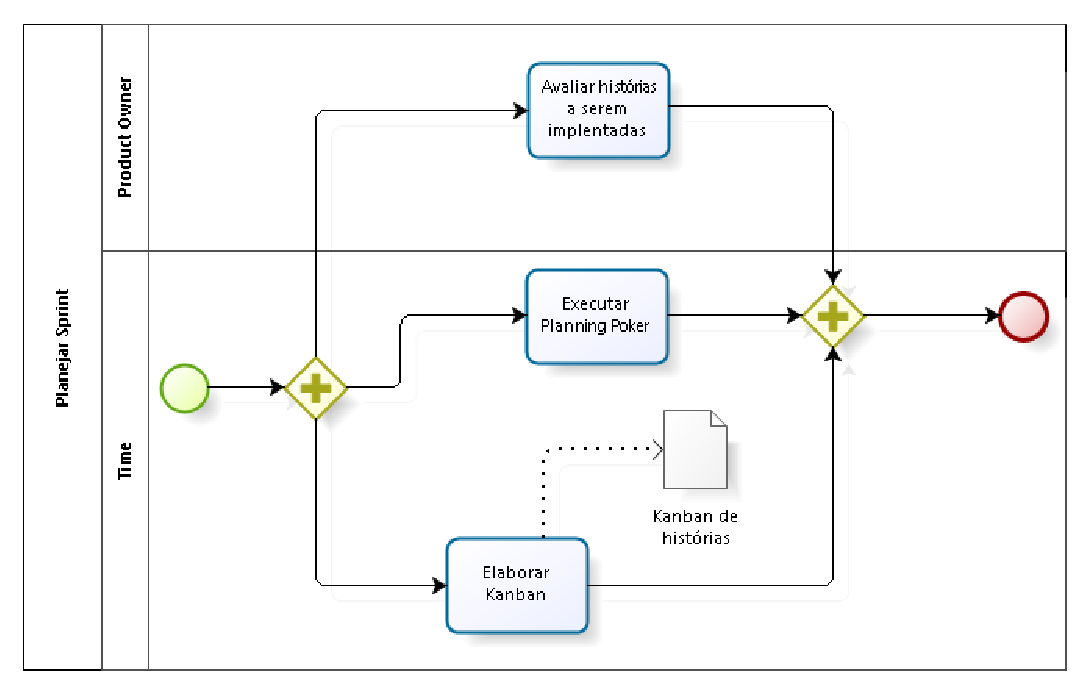
\includegraphics[keepaspectratio=true,scale=0.6]{figuras/processoPlanejar.eps}
    \caption[Planejar sprint]{Processo - Nível de Time - Planejar sprint}
\end{figure}

\subsection{Reunião 04}
Foi feita uma reunião interna, somente com os membros da equipe de requisitos, para realizar o planejamento da sprint 01, foi analisado com base na prioridade determinada pelo PO de qual épico e feature as histórias de usuários seriam selecionadas para serem implementadas. Foi levado em consideração também a produtividade e perfil da equipe. Com base nesses critérios, foram determinados as histórias de usuário a serem implementadas. 

Sendo estas as histórias de usuário, do business EP01 das features Business FT01 e Enable FT02 \ref{featuresss} selecionadas para serem implementadas: 

 \indent \textbf{Nome:} Inserir dados pessoais\\
 \indent \textbf{Prioridade:} Altíssima\\
 \indent \textbf{Identificador:} US01\\
 \indent \textbf{Descrição:} Eu, como membro da empresa, quero inserir informações relativas aos meus dados pessoais, para permitir que à empresa me conheça melhor.\\

 \indent \textbf{Nome:} Visualizar dados dos usuários\\
 \indent \textbf{Prioridade:} Alta\\
 \indent \textbf{Identificador:} US02\\
 \indent \textbf{Descrição:} Eu, como membro, desejo visualizar os as informações pessoais de outros membros para que eu consiga ter o contato dos demais membros.\\

 \indent \textbf{Nome:} Modificar perfis dos membros\\
 \indent \textbf{Prioridade:} Altíssima\\
 \indent \textbf{Identificador:} US 01\\
 \indent \textbf{Descrição:} Eu, como gestor de pessoas, desejo que os membros da empresa sejam diferenciados pelo perfil para que eles possam ter permissões de acessos diferenciadas a certo conteúdos.\\

 \indent \textbf{Nome:} Gerar novo usuário\\
 \indent \textbf{Prioridade:} Alta\\
 \indent \textbf{Identificador:} US02\\
 \indent \textbf{Descrição:} Eu, como gestor de pessoa, quero poder cadastrar membros no sistema para que eles possam usufruir dos recursos do software.\\
             
 \indent \textbf{Nome:} Login e logout\\
 \indent \textbf{Prioridade:} Alta\\
 \indent \textbf{Identificador:} US05\\
 \indent \textbf{Descrição:} Eu como membro desejo inserir meus dados de login para que eu possa ter acesso ao sistema.\\

Com as histórias de usuário selecionadas, foi realizado o plannig poker e foi determinado que a história de Visualizar dados dos usuários \ref{codigoimg} seria nosso parâmetro para definir complexidade da história, sendo esta equivalente ao ponto 01, baseando-se nas experiências dos membros da equipe de requisitos. Logo, as pontuação das histórias foram: 

\begin{table}[H]
    \centering
    \label{historiasImplementar}
    \caption{Histórias pontuadas para implementação}
    \begin{tabular}{|l|l|}
        \hline
        US & Pontuação\\
        \hline
        Inserir dados pessoais &  02\\
        \hline
        Visualizar dados dos usuários & 01\\
        \hline
        Modificar perfis dos membros & 03\\
        \hline
        Gerar novo usuário & 02\\
        \hline 
        Login / logout & 02\\
        \hline
    \end{tabular}
\end{table}

\section{Execução da sprint}
\begin{figure}[H]
    \centering
    \label{identificarExecutar}
    \includegraphics[keepaspectratio=true,scale=0.6]{figuras/processoExecutar.eps}
    \caption[Executar sprint]{Processo - Nível de Time - Executar sprint}
\end{figure}
